\documentclass[fleqn,12pt]{olplainarticle}
\usepackage{graphicx}
\graphicspath{ {./} }
% Use option lineno for line numbers 
\renewcommand{\baselinestretch}{1.3}

\title{Docker in Software Architecture}

\author[1]{Daniel Koch}
\author[2]{Sebastian Sergelius}
\affil[1]{daniel.koch@helsinki.fi}
\affil[2]{sebastian.sergelius@helsinki.fi}

\keywords{docker, software architecture, containers}

\begin{abstract}
Please provide an abstract of no more than 300 words. Your abstract should explain the main contributions of your article, and should not contain any material that is not included in the main text. 
\end{abstract}

\begin{document}
\flushbottom
\maketitle
\thispagestyle{empty}
\pagebreak
\tableofcontents
\section{Introduction}

With the rise of DevOps and the use of Docker, containerization has become more and more relevant to think about even in software architecture. DevOps does not have any official definition.
One formal definition is given by \cite{Jabbari_devops}: 
\begin{displayquote}
"DevOps is a development methodology aimed at bridging the gap between Development and Operations, emphasizing communication and collaboration, continuous integration, quality assurance and delivery with automated deployment utilizing a set of development practices".
\end{displayquote}
Another way to put DevOps is that it consists of the development of software and operations and that DevOps means that development, release, configuration, and monitoring are all done by the same people, rather than having separate teams for every part \citep{hy:DevOps_with_Docker}.

Containerization is common as a part of DevOps. Docker is one of the most common containerization software since its release in 2013 \citep{aquasec:orchestration}. In this technology brief, we will explain what is meant by containerization, how it compares to virtual machines and how do you use docker as a part of software architecture.


\section{overview of the main functional features (what does it do for you?) if applicable}

Tähän varmaan siitä virtuaalikoneista vs kontit, kuten miten se abstrahoi os level vs hardware?

\section{Docker Architecture}

In this section we will be discussing the Docker architecture and its vital components that builds the technology under study. The Docker architecture is based on a client-server model where the client is called Docker client and the server is called Docker Host \citep{docker:overview, aquasec:docker_architecture}. The client and the host do not necessarily need to be on the same system, as the client can communicate with the host using the Docker REST API through either a UNIX socket or a network interface. Docker images are written in a Dockerfile, which defines the steps how to build and run the image in a container. These built images can be stored in a private or public Docker Registry.

\begin{figure}[h]
    \centering
    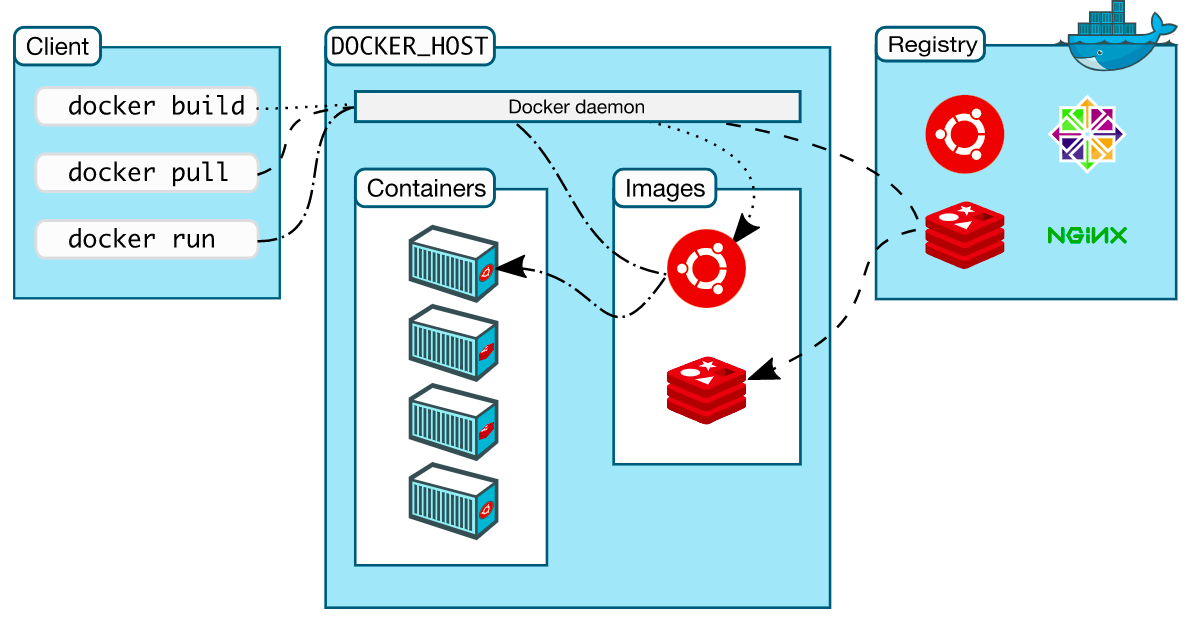
\includegraphics[width=1\textwidth]{docker-overview}
    \caption{Overview of the Docker Architecture\cite{docker:overview}}
    \label{fig:overview}
\end{figure}

\subsection{Docker Client}

The Docker Client is the application that the user uses to interact with the Docker environment \cite{aquasec:docker_architecture}. The client provides a command line interface (CLI) that enables the user to give commands to the Docker Hosts daemon. A client is able to communicate with many daemons.

\subsection{Docker Host}

The Docker host contains of many components, such as the daemon, images, containers, networking and storage, that provides the environment for running and executing applications \citep{aquasec:docker_architecture}. The daemon is responsible for handling container related commands that are received from the client, such as pulling pre-built images from a registry, executing instructions defined in a Dockerfile and building and running the containers on the server.

\subsubsection{Docker Images}

Docker Images are read-only binary files that are used to build containers \citep{docker:overview}. Images are built using a Dockerfile that defines the instructions for the daemon to execute. Each instruction creates a layer in the image built. If an instruction is changed in the Dockerfile the daemon will only rebuild the image on the layers affected by the change. Once the image is built, you can run the image in a container. Each container can be saved as an image and images support versioning.

\subsubsection{Docker Containers}

Docker Containers are isolated environments which runs applications \citep{aquasec:docker_architecture}. The container contains all the necessary dependencies that are required for running the application. Running containers are isolated from other containers and also have a good isolation from the host machine \citep{docker:security}. Containers can be connected to networks and storages.

\subsubsection{Docker Networking}

Docker uses \textit{iptables} rules on Linux hosts to provide network isolation \citep{docker:iptables}. Linux iptables provides the possibility to restrict access for the Docker host, as by default, all external IPs are able to connect to a Docker host. Docker environment has several network drivers by default, such as \citep{docker:network}:

\begin{itemize}
    \item \textbf{bridge}: The default driver. Used when multiple containers on the same host need to communicate with eachother.
    \item \textbf{host}: Containers use the Docker host's networking directly.
    \item \textbf{overlay}: Used to connect multiple Docker daemons together. Should be used if two containers are on different Docker hosts.
    \item \textbf{none}: Disables container networking.  
\end{itemize}

Docker also supports third-party network plugins, user-defined IP addressing and defining a MAC address to a container, so the container can be seen as a physical host in the network \citep{docker:network}.

\subsubsection{Docker Storage}

Data stored within the container are non-persistent and the data will disappear once the container stops running \citep{aquasec:docker_architecture}. For persistent storage Docker offer four options – Data Volumes, Data Volume Container, Directory Mounts and Storage plugins. Data volumes are located on the hosts file system and can be shared with many containers. A data volume container is a dedicated container that hosts a volume from the host. Each container using the volume connects to the container that hosts the persistent storage. Using Directory mounting, a container can have access to any folder on the host and with storage plugins containers can use persistent storage that is for example hosted on the cloud.

\subsection{Docker Registry}

A Docker registry is a service for storing and downloading images \citep{aquasec:docker_architecture}. A registry can be publicly or privately hosted. Some most known public registries are Docker Hub and Docker Cloud.

\section{Quality Attributes}

The qualities (-ilities) that the TUS claims to support (what?) and justifications for the claims (how?)

Based on how Docker is built, the system has some qualities hoisted in it. In this section, we will list some important qualities from the architectural and agile perspective, if you decide to use Docker in your infrastructure. 

\subsection{Portability}
One key aspect of Docker is its Portability. With software portability, we refer to the usability of the same software in different environments, such as the underlying operating system or hardware \citep{wiki:Software_portability}. Portability is achieved based on how the Docker technology is built. Each container includes all the dependencies required for the application to work and only requires an underlying operating system and infrastructure that supports the Docker Engine \citep{hy:DevOps_with_Docker}.

\subsection{Deployability}
As Docker images are versionable, this gives the possibility to easily test, roll back and deploy applications\cite{hentsu:benefits}. As Docker images are smaller then Virtual Machine images, deploying an image to production is fast and results in a short downtime in a production environment. 

\subsection{Security}
There was a paper about this in IEEE iirc, going to find it later. But at least with docker, your software is isolated from other software.

\subsection{Scalability}
Scalability is one of the main selling points of Docker and especially if bundled with microservice architecture the scalability is great. With Docker, you can easily deploy as many containers of your service as you need and even adjust the number of containers during runtime.

\subsection{Maintainability}
Docker separates all applications into their own virtual environments. With this, different applications don't interfere with other applications and each application can have all its dependencies easily and reliably every time without affecting other software. This allows different applications to use different versions of the same dependencies.

\section{Architectural impact}

What aspect of application/system architecture is affected by using it and how?

\section{Limitations}

What is it not suited for (any inherent limitations or reported issues)?

\section{Docker Tools}

Tool support / automation provided (can be also from 3rd parties) to help application developers be more productive

\section{Acknowledgments}

Additional information can be given in the template, such as to not include funder information in the acknowledgments section.

\bibliography{sample}

\end{document}